The performances of the developed models were assessed using the \gls{mcrmse}. The final Kaggle scores, representing the Ensemble Models' performance and generalization capabilities, are as follows:

\begin{itemize}
    \item \textbf{Final Public Score:} 0.4956
    \item \textbf{Final Private Score:} 0.4977
\end{itemize}
% \begin{figure}[h]
% 
\includegraphics[keepaspectratio, width=\textwidth]{final_score_kaggle.png}
% \caption{Final Kaggle Score}
% \label{fig:rouge-correlation-matrix}
% \end{figure}
Furthermore, the Ensemble Model was evaluated on a separate test set, with scores during training and testing phases:

\begin{itemize}
    \item \textbf{Final Training-Set Score:} 0.3687
    \item \textbf{Final Test-Set Score:} 0.4981
\end{itemize}

\subsubsection{Evolution of Kaggle Scores}

The following graphs
(\hyperref[fig:kaggle-score-evolution]{Figure~\ref{fig:kaggle-score-evolution}}
and
\hyperref[fig:kaggle-score-evolution_clipped]{Figure~\ref{fig:kaggle-score-evolution_clipped}})
illustrate the evolution of Kaggle scores throughout the development process. Some models, like the RNN and LSTM are not listed as they were not tested thoroughly, and those with multiple entries have some variation in their hyperparameters. The full range and a clipped version of the graph - highlighting the lowest (best) scores - show the progress of the models and their performances.

\begin{figure}[H]
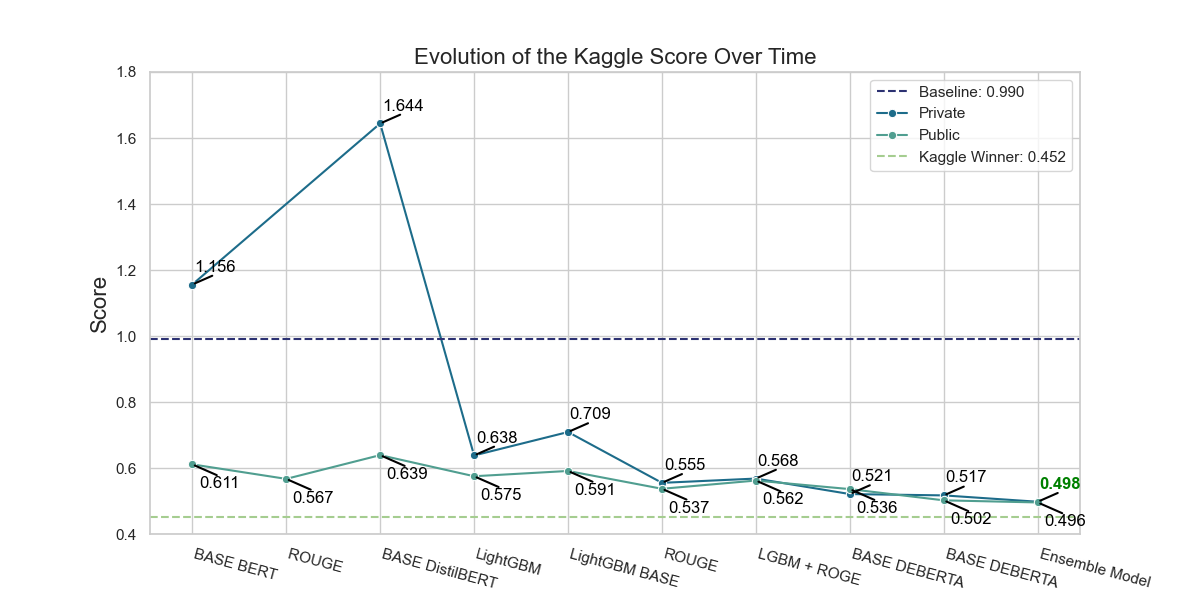
\includegraphics[keepaspectratio, width=\textwidth]{Kaggle_Score_Evolution_(Full).png}
\caption{Kaggle Score Evolution}
\label{fig:kaggle-score-evolution}
\end{figure}
\begin{figure}[H]
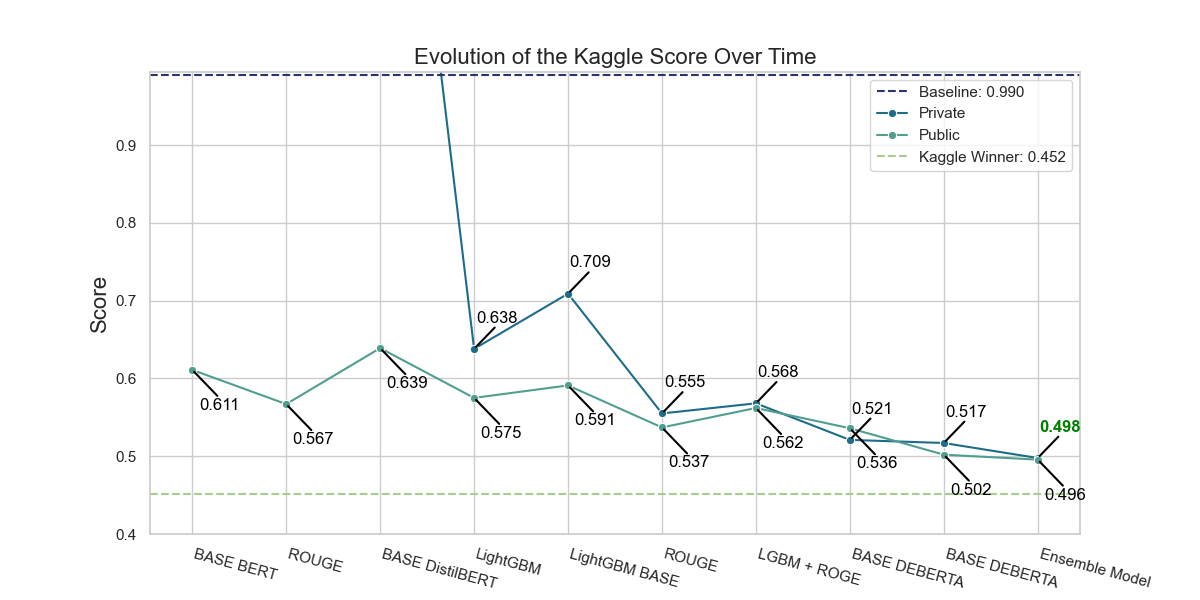
\includegraphics[keepaspectratio, width=\textwidth]{Kaggle_Score_Evolution_(Clipped_1).png}
\caption{Kaggle Score Evolution (Clipped at the Baseline score)}
\label{fig:kaggle-score-evolution_clipped}
\end{figure}
